\section{計算領域(格子数・解像度・MPIプロセス数)の指定}
\label{sec:domain}
%=======================================================================

水平格子間隔と格子数が計算領域を決定するのは言うまでもないが、
SCALEではMPIプロセス数も考慮する必要がある。
図X%\ref{fig:domain}
は、計算領域、及び、水平格子間隔、格子数、MPIプロセス数の関係を示している。
%図から明らかなように、計算領域は
それぞれの設定方法については、次節以降で説明する。

%\begin{figure}[h]
%\begin{center}
%  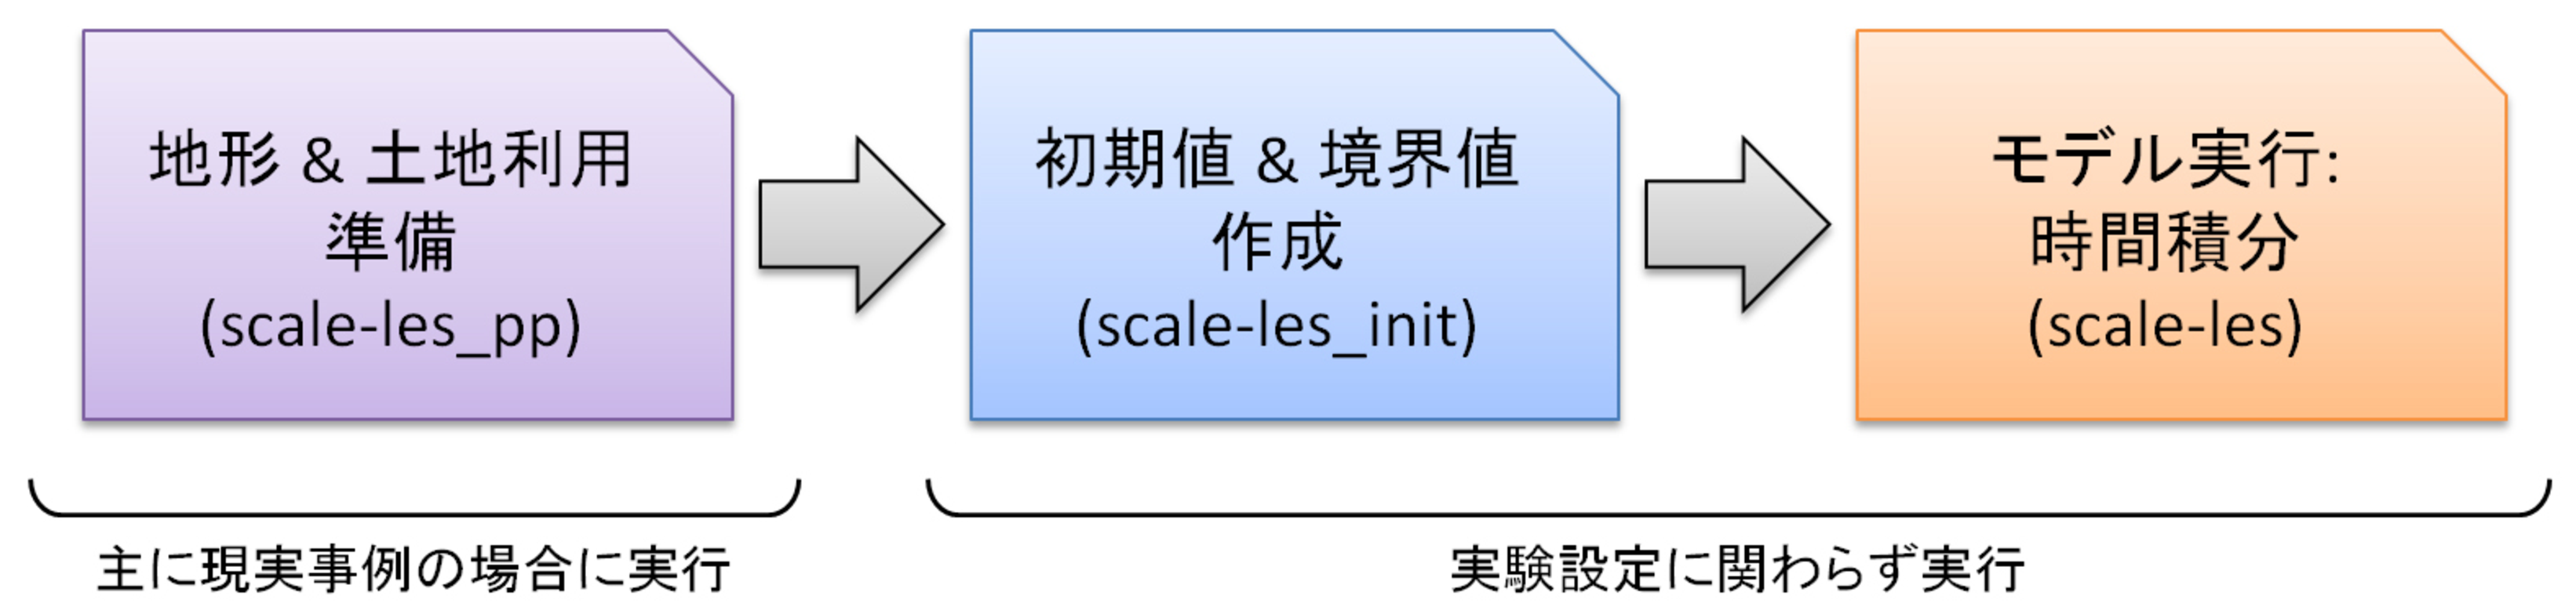
\includegraphics[width=0.9\hsize]{./figure/how_to_run.eps}\\
%  \caption{SCALE-RMモデルの実行過程}
%  \label{fig:howto}
%\end{center}
%\end{figure}

\subsection{計算領域の大きさ} \label{sec:adv_domainsize}
%------------------------------------------------------
ここで説明する\textcolor{red}{\bf 計算領域の設定は、pp\_***.conf、init\_***.conf、run\_***.confの
configファイルの間で必ず一致させなければならない。}このことに注意して設定変更を進めてもらいたい。

SCALEはMPI並列プログラムであり、全計算領域は複数のMPIプロセスに分割されて並列実行される。計算領域は
水平2次元(東西方向 $\times$ 南北方向)に分割される。したがって計算領域の大きさは、MPIプロセス数と
1つのMPIプロセスが担当する格子点数によって決まる。以降、X方向は水平軸の東西方向、Y方向は水平軸の南北方向を
それぞれ意味するものとする。

X方向、およびY方向のMPIプロセスの割付設定は、configファイルの\verb|PARAM_PRC|の項目にある\verb|PRC_NUM_X|、
および\verb|PRC_NUM_Y|よって指定される。また、1つのMPIプロセスが担当する格子点数は、
\verb|PARAM_INDEX|項目にある\verb|KMAX|、\verb|IMAX|、\verb|JMAX|の変数によって指定され、
それぞれ鉛直方向、X方向、Y方向の格子点数を表す。
したがって、X方向の総格子点数は\verb|PRC_NUM_X| $\times$ \verb|IMAX|、Y方向の総格子点数は
\verb|PRC_NUM_Y| $\times$ \verb|JMAX|と表現される。また、計算に必要な総MPIプロセス数は、
\verb|PRC_NUM_X| $\times$ \verb|PRC_NUM_Y|となる。実行時にMPIコマンドに指定するMPIプロセス数は、
この総MPIプロセス数を指定しなければならない。この条件を満たさない場合は,LOGファイルなどに\\

\noindent {\small {\gt
\ovalbox{
\begin{tabularx}{140mm}{l}
\verb|xxx total number of node does not match that requested. Check!| \\
\end{tabularx}
}}}\\

\noindent というメッセージが出力がされて計算が異常終了するので、設定、もしくは実行コマンドを見なおしてもらいたい。

ここまでの復習として、現実大気実験のチュートリアルで使用した\verb|run.conf|ファイルを例にして、
上述の内容を確認してみる。\\

\noindent {\small {\gt
\ovalbox{
\begin{tabularx}{140mm}{l}
\verb|&PARAM_PRC| \\
\verb| PRC_NUM_X      = 2,| \\
\verb| PRC_NUM_Y      = 2,| \\
\verb| PRC_PERIODIC_X = .false.,| \\
\verb| PRC_PERIODIC_Y = .false.,| \\
\verb|/| \\
 \\
\verb|&PARAM_INDEX| \\
\verb| KMAX = 36,| \\
\verb| IMAX = 60,| \\
\verb| JMAX = 60,| \\
\verb|/| \\
\end{tabularx}
}}}\\

\noindent まずMPIプロセス数については\verb|PRC_NUM_X = 2|、\verb|PRC_NUM_Y = 2|と設定されているため、
X方向、Y方向ともに2分割されており、総計として4つのMPIプロセスを使用した計算となることがわかる。
一方、1つのMPIプロセスあたりの格子点数については、\verb|IMAX = 60|、\verb|JMAX = 60|と指定されているため、
総格子点数としては、X方向、Y方向ともに$2 \times 60 = 120$となり120格子点である。
同じconfigファイル内に記載されている\verb|PARAM_GRID|の項目の\verb|DX|、\verb|DY|はともに15000 m(15 km)
と指定されているため、120 grid $\times$ 15 km = 1800 km の計算から、1800 km $\times$ 1800 km の正方形の計算領域
が設定されていることがわかる。

\verb|PARAM_TIME|の項目の\verb|PRC_PERIODIC_X|、\verb|PRC_PERIODIC_Y|は側面境界条件に関する設定である。
その詳細は次節で説明する。



\subsection{MPIプロセス数}
ここでは、第\ref{sec:tuto_ideal}章の実験設定を例に、
実行時のMPIプロセス数の変更方法について説明する。
%
先に述べた通り、SCALEの入出力ファイルは、MPIプロセス毎に分割されている。
そのため、MPIプロセス数を
変更すると分割ファイル数も必ず変わることになる。
従って、2-MPI並列用に作成した初期値ファイルは、
4-MPI並列のモデル実行には使用できない。
MPIプロセス数を変更するには、
``\verb|init_***.conf|''、
``\verb|run_***.conf|''の両方を編集・変更し、
再度初期値作成から行わなければならない。

MPIプロセス数は、
\verb|init_R20kmDX500m.conf|や\verb|run_R20kmDX500m.conf|の
``\verb|PARAM_PRC|''で指定する。
%
第\ref{sec:tuto_ideal}章で使用した\verb|init_R20kmDX500m.conf|は
下記の設定となっている。\\

\noindent {\small {\gt
\ovalbox{
\begin{tabularx}{140mm}{l}
\verb|&PARAM_PRC|\\
\verb| PRC_NUM_X       = 2,|\\
\verb| PRC_NUM_Y       = 1,|\\
\verb|/|\\
\end{tabularx}
}}}\\

``\verb|PRC_NUM_X|''は X方向(東西方向)のMPI並列分割数、
``\verb|PRC_NUM_Y|''は Y方向(南北方向)のMPI並列分割数である。
全MPIプロセス数は、${PRC}_{total}={PRC}_{X} \times {PRC}_{Y}$ となり、
上記の設定では、X方向に2分割、Y方向に1分割(分割なし)の2-MPI並列ということになる。



\subsection{水平格子数}
%-----------------------------------------------------------------------

格子数の設定は、configureファイルの
``\verb|PARAM_INDEX|''で行う。


\noindent {\small {\gt
\ovalbox{
\begin{tabularx}{140mm}{l}
\verb|&PARAM_INDEX|\\
\verb| KMAX = 97,|\\
\verb| IMAX = 20,|\\
\verb| JMAX = 2,|\\
\verb|/|\\
\end{tabularx}
}}}\\

\verb|KMAX、IMAX、JMAX|は、
鉛直層数、X方向の格子点数、Y方向の格子点数をそれぞれ意味する。
ただし、IMAXとJMAXは、MPIプロセス当たりの
値であることに注意が必要である。
つまり、計算領域全体での格子点数は、
\begin{eqnarray}
東西方向:{Grids}_{X}={\bf IMAX} \times {\bf PRC}_{X} \nonumber \\
南北方向:{Grids}_{Y}={\bf JMAX} \times {\bf PRC}_{Y} \nonumber 
\end{eqnarray}
となる。
鉛直方向には分割しないため、\verb|KMAX|がそのまま領域全体の鉛直層数を表す。
従って、このチュートリアルの全体の格子点数は、X方向(東西)に40点、Y方向(南北)に2点、
そして鉛直に97層ということになる。


さて、上記の設定を変更して4-MPI並列で実行できるようにしてみる。注意する点は領域全体の格子点数を
維持するように設定することである。今回は準2次元実験なので、X方向に4分割して4-MPI並列を達成する。
この場合の設定方法は下記のとおりである。\\

\noindent {\small {\gt
\ovalbox{
\begin{tabularx}{140mm}{l}
\verb|&PARAM_INDEX|\\
\verb| KMAX = 97,|\\
\verb| IMAX = 10,|\\
\verb| JMAX = 2,|\\
\verb|/|\\
\\
\verb|&PARAM_PRC|\\
\verb| PRC_NUM_X       = 4,|\\
\verb| PRC_NUM_Y       = 1,|\\
\verb|/|\\
\end{tabularx}
}}}\\

\noindent X方向に4分割を指定するため、\verb|PRC_NUM_X = 4|と記述されている。そして、領域全体で40格子点
とするために、\verb|IMAX = 10|と記述されている。Y方向と鉛直方向には何も変更していない。
\textcolor{red}{この変更を、{\bf init\_R20kmDX500m.conf}と{\bf run\_R20kmDX500m.conf}の両方に施さなければならない。}
そして、つぎのようにMPIコマンドに指定するプロセス数を``4''として、初期値作成、モデル実行の順で
作業を進めれば、4-MPI並列で実行することができる。
\begin{verbatim}
  $ mpirun  -n  4  ./scale-rm_init  init_R20kmDX500m.conf
  $ mpirun  -n  4  ./scale-rm       run_R20kmDX500m.conf
\end{verbatim}

計算領域(総演算量)を維持したままMPIプロセス数を
2倍に増やすことによって、プロセス数に応じて使用するコア数も
2倍となる場合、1つのMPIプロセスあたりの
問題サイズ(演算量 per PRC)が1/2に減る。
したがって、計算にかかる時間も理想的には半分になる
%\footnote{計算科学用語では、この変更、つまり総演算量一定でプロセスあたりの演算量を減らしていくことを``strong scaling''と呼ぶ。}。
実験機では、2-MPI並列のときチュートリアルの時間積分に60 sec かかっていたが、4-MPI並列にすることで同じ計算が32 secで終了できた。
ここで説明したMPIプロセス数の変更を加えたサンプルファイルが、同じディレクトリ下の``sample''ディレクトリ内に
\verb|init_R20kmDX500m.pe4.conf|、\verb|run_R20kmDX500m.pe4.conf|として置いてあるので、うまく実行できない場合は
参考にして欲しい。



\subsection{水平・鉛直格子間隔}
%-----------------------------------------------------------------------
SCALEでは、格子点の位置を均等間隔に設定することも、
任意の格子点位置を直接指定することもできる。
以下で説明する
\textcolor{red}{\bf 格子間隔の設定は、pp\_***.conf、init\_***.conf、run\_***.confの
configファイルの間で一致させなければならないことに注意が必要である。}


\subsubsection{均等間隔で設定する場合}
%-----------------------------------------------------------------------&
configファイルの\verb|PARAM_GRID|の\verb|DX|、\verb|DY|、\verb|DZ|に
それぞれ、東西、南北、鉛直方向の格子間隔を指定する。

\noindent {\small {\gt
\ovalbox{
\begin{tabularx}{140mm}{lX}
\verb|&PARAM_GRID  | & \\
\verb| DX = 500.D0,| & ; X方向(東西方向)の格子間隔\\
\verb| DY = 500.D0,| & ; Y方向(南北方向)の格子間隔\\
\verb| DZ = 500.D0,| & ; Z方向(鉛直方向)の格子間隔\\
\verb|/|\\
\end{tabularx}
}}}\\




\subsubsection{任意の格子点位置を指定}
%-----------------------------------------------------------------------&
SCALEの格子系はArakawa-Cグリッド、
およびLorenzグリッドであるため、水平方向と鉛直方向ともに
スタッガード点(1/2ずれた点)に位置する変数がある。
コントロールボリュームに対して中心点に位置する格子点を
Center Pointと呼び、コントロールボリュームの面に位置する格子点
(Center Pointに対して1/2ずれている)をFace Pointと呼ぶ。
そして、これらの頭文字と方向を組み合わせて\verb|CX、CY、CZ|や\verb|FX、FY、FZ|と呼ぶ
(図\ref{fig:scale_grid})

\begin{figure}[h]
\begin{center}
  \includegraphics[width=0.8\hsize]{./figure/Center-Face.eps}\\
  \caption{SCALE-RMの格子の定義}
  \label{fig:scale_grid}
\end{center}
\end{figure}


直接格子点の位置を指定する場合は、Center PointもしくはFace Pointの
位置を明記すれば良い。
これらの変数の単位はメートル[m]である
\footnote{指定の際には、
シミュレーションの計算精度(モデルのコンパイル時に指定した浮動小数点の精度。
デフォルトでは倍精度)を用いることが望ましい。}


例として理想実験のチュートリアルのrun.confファイル
(run\_R20kmDX500m.conf)を下記に示す。\\

\noindent {\small {\gt
\ovalbox{
\begin{tabularx}{140mm}{l}
\verb|&PARAM_GRID|\\
\verb| DX = 500.D0,|\\
\verb| DY = 500.D0,|\\
\verb| FZ(:) = |\\
\verb|    80.000000000000000      ,|\\
\verb|    168.00000190734863      ,|\\
\verb|    264.80000610351567      ,|\\
\verb|     〜 中略 〜|\\
\verb|    14910.428862936289      ,|\\
\verb|    15517.262523292475      ,|\\
\verb|    16215.121232702089      ,|\\
\verb|    17017.658748523147      ,|\\
\verb|    17940.576891717363      ,|\\
\verb|    19001.932756390710      ,|\\
\verb|    20222.492000765058      ,|\\
\verb| BUFFER_DZ = 5000.D0,|\\
\verb| BUFFFACT  =   1.0D0,|\\
\verb|/|\\
\end{tabularx}
}}}\\

%\verb|DX|、\verb|DY|は``\verb|500.D0|''と倍精度表記を用いて500 mと指定されており、
%水平方向の格子間隔は500 mの均等間隔に設定されていることがわかる。
%一方、
\verb|FZ(:)|の項目は鉛直方向の格子点位置を直接指定している。
ここには示していないが、同じconfigファイル中の
\verb|PARAM_INDEX|の項目に
``\verb|KMAX = 97|''として鉛直97層であると設定されているため、
最下層から再上層まで97層分の位置が指定されている。
これを見れば、最下層の高度は80 m、最上層の高度は約20 kmであるとわかる。
モデルの鉛直層とり方を変えたい場合は、
これに習って\verb|KMAX|で指定した層数に応じて高度を指定すればよい
\footnote{独自の鉛直層設定の作成をサポートするツールとして、scale/scale-rm/util/makevgridのディレクトリ下に
``make\_vgrid.f90''というFortranプログラムといくつかのサンプルnamelistが用意されている。これをコンパイルして
実行すれば直ちにconfigファイルに貼り付けて使用できるフォーマットになった鉛直層設定を作成できる。}
。



%\section{実験設定の詳細} \label{sec:adv_settings}
%====================================================================================

%ここではチュートリアルで触れなかった実験設定の詳細について説明する。SCALEでサポートする全てを
%網羅してはいないが、格子間隔、計算領域、積分時間間隔、物理過程等の重要な設定方法については
%できる限り丁寧に説明するように心がけた。実験設定は全て、\verb|pp_***.conf|、\verb|init_***.conf|、
%および\verb|run_***.conf|のconfigファイルを編集することで設定できる。従って、以降の説明は
%全てconfigファイルの編集方法について述べたものである。configファイルの設定変数の詳細は
%付録\ref{app:namelist}に記載があるので、本節と併せて読み進めて欲しい。
%また以下の説明は、第3章と第4章のチュートリアルをすでに実行してきたものとして説明する。



\subsection{バッファー格子点の設定}
%-----------------------------------------------------------------------
SCALEでは計算領域境界のすぐ内側に「バッファー格子点」を設定することができる。バッファー格子点では、指定された値や
親モデルのデータにダンピングする、いわゆるナッジングが行われる。これは、モデル最上層で重力波が反射することを
緩和するための「スポンジ層」として利用したり、現実大気実験を行う際に側面境界において親モデルと
SCALEで計算される大気場が乖離することを防ぐための「緩和領域」として利用される。

バッファー格子点は、\verb|BUFFER_DX|、\verb|BUFFER_DY|、\verb|BUFFER_DZ|、および\verb|BUFFFACT|の変数によって
設定される。\verb|BUFFER_DX|、\verb|BUFFER_DY|、\verb|BUFFER_DZ|は、それぞれの方向のバッファー領域の幅
(単位はメートル)を示す。バッファー領域は境界から内側に\verb|BUFFER_DX|等で指定された幅で設置され、
バッファー領域内の格子点はバッファー格子点として認識される。したがって、その分だけナッジングの影響を受けないで計算
される自由領域は狭くなることに注意が必要である。水平方向には東西南北どの方向にも同様にバッファー領域が設定されるが、
鉛直方向には計算領域の上端にのみバッファー領域が設定され、下端には設定されない。
\verb|BUFFFACT|はバッファー領域内の格子点の格子間隔に対するストレッチ係数である。
下記の関係式によって、バッファー領域内の格子間隔(BDX)は決定される。
\begin{eqnarray}
BDX_{i+1}&=&{BDX_{i}}^{BUFFFACT} \nonumber \\
BDX_{1}&=&DX_{default} \nonumber
\end{eqnarray}
ここで、$i$はバッファー領域内の格子点番号を表し、
計算領域の内側から外側へ向かって番号が振られる。
$DX_{default}$は\verb|PARAM_GRID|の項目で設定される
元々の\verb|DX|を意味する。
$i$の最大値$n$は、$\sum_{i=1}^n BDX_{i} > BUFFER_{DX}$の関係を達成する最小の数として決定される。
したがって、``\verb|BUFFFACT = 1.0|''ならば、格子間隔をストレッチせずに等間隔であることを意味し、
``\verb|BUFFFACT = 1.2|''ならば、計算領域の内側から境界へ向けて、格子点間距離がもともとの格子間隔から
1.2倍の割合で広がっていくことを意味する。\verb|BUFFFACT|の値を大きくすると、バッファー領域の幅が同じでも
バッファー格子点として使用される格子点数は少なくなる。

例として理想実験のチュートリアルのrun.confファイル(run\_R20kmDX500m.conf;上に表示したもの)を見てみると、
\verb|BUFFER_DZ = 5000.D0|、\verb|BUFFFACT = 1.0D0|と指定されている。\verb|BUFFER_DZ|以外には指定がないので、
水平方向にはバッファー領域が設定されない(この実験は水平方向には周期境界条件になっておりバッファー領域は必要ない)。
\verb|BUFFFACT = 1.0D0|となっているため、もとの格子間隔のままストレッチは行わない。
最上層の高度が20222 mと指定されており、鉛直方向のバッファー領域の幅は5000 mと指定されているため、
モデル計算領域のトップから高度15222 mまでがバッファー領域となる。鉛直層の高度指定によれば、92層目の高度が
15517 mで、91層目の高度が14910 mであるため、92層目まではバッファー領域だが、91層目はバッファー領域ではない。
繰り返しになるが、これらの設定は\verb|pp_***.conf|、\verb|init_***.conf|、\verb|run_***.conf|の
すべてのconfigファイルにおいて共通した設定になっていなければならない。

SCALEでは、バッファー領域の大きさ、バッファー格子点の数について、まだ明確な指標を設定できていないが、
鉛直方向(計算領域トップ)のバッファー格子点は5点以上、水平方向(側面境界付近)のバッファー格子点は
20〜40点程度を推奨している。実験設定や事例によっては、さらにバッファー格子点を増やしたり、ストレッチ係数を
用いてバッファー領域を広げる処理が必要であったり、ここでは説明しなかったが\verb|ATMOS_BOUNDARY_taux|、
\verb|ATMOS_BOUNDARY_tauy|といった設定項目を調整してバッファー領域のナッジング強度を強める必要があったりする。




\subsection{計算領域の変更の練習問題}
ここでは、現実大気実験のチュートリアルのconfigファイル(\verb|run.conf|)を元にしていくつかの変更例を説明する。
以下の変更例をもとに、自分の行いたい実験設定にあったconfigファイルを作り上げてもらいたい。\\


{\bf a. MPIプロセス数はそのままに計算領域を4倍に広げる}\\

この設定はとても簡単である。デフォルト設定は、X方向、Y方向ともに2つのMPIプロセスを使用し、格子点数はともに
30点なので、全領域の格子点数は、$(2 \times 60)_{x} \times (2 \times 60)_{y} = 14400$点である。
従って、計算領域を4倍に広げるためには、\verb|IMAX|、\verb|JMAX|の値をデフォルトに対して2倍の値に変更するだけである。
これで、全領域の格子点数は、$(2 \times 120)_{x} \times (2 \times 120)_{y} = 57600$点となり、14400点の4倍の
計算領域になっている。この変更を施したconfigファイルの例は次のとおりである。
赤文字の部分がデフォルトからの変更点を意味する。\\

\noindent {\small {\gt
\ovalbox{
\begin{tabularx}{140mm}{l}
\verb|&PARAM_PRC| \\
\verb| PRC_NUM_X      = 2,| \\
\verb| PRC_NUM_Y      = 2,| \\
\verb| PRC_PERIODIC_X = .false.,| \\
\verb| PRC_PERIODIC_Y = .false.,| \\
\verb|/| \\
 \\
\verb|&PARAM_INDEX| \\
\verb| KMAX = 36,| \\
\textcolor{red}{\verb| IMAX = 120,|} \\
\textcolor{red}{\verb| JMAX = 120,|} \\
\verb|/| \\
\end{tabularx}
}}}\\

\vspace{5mm}
{\bf b. 1つのMPIプロセスあたりの格子点数はそのままに計算領域を4倍に広げる}\\

先程は、MPIプロセス数を維持して計算領域を広げたが今度は、1つのMPIプロセスあたりの格子点数はそのままに、MPIプロセス数を
増やすことで計算領域を4倍に広げる方法を説明する。1つのMPIプロセスあたりの格子点数(プロセスあたりの演算量)は
そのままにMPIプロセス数を増やすことで計算領域を広げる(総演算量を増やす)。この場合、1つのCPUが担当する問題サイズは
変わらないため、理想的には計算にかかる時間を増やすことなく計算領域を広げることができる
\footnote{計算科学用語では、この変更、つまりプロセスあたりの演算量一定で総演算量を増やしていくことを``weak scaling''と呼ぶ。}。

計算領域を4倍に広げるためには、\verb|PRC_NUM_X|、\verb|PRC_NUM_Y|の値をデフォルトに対して2倍の値に変更するだけである。
これで、全領域の格子点数は、$(4 \times 60)_{x} \times (4 \times 60)_{y} = 57600$点となり、14400点の4倍の
計算領域になっている。このとき必要なMPIプロセス数は、$4 \times 4 = 16$プロセス、つまりデフォルトの4倍のMPIプロセス数が必要になる。
この変更を施したconfigファイルの例は次のとおりである。赤文字の部分がデフォルトからの変更点を意味する。\\

\noindent {\small {\gt
\ovalbox{
\begin{tabularx}{140mm}{l}
\verb|&PARAM_PRC| \\
\textcolor{red}{\verb| PRC_NUM_X      = 4,|} \\
\textcolor{red}{\verb| PRC_NUM_Y      = 4,|} \\
\verb| PRC_PERIODIC_X = .false.,| \\
\verb| PRC_PERIODIC_Y = .false.,| \\
\verb|/| \\
 \\
\verb|&PARAM_INDEX| \\
\verb| KMAX = 36,| \\
\verb| IMAX = 60,| \\
\verb| JMAX = 60,| \\
\verb|/| \\
\end{tabularx}
}}}\\

\vspace{5mm}
{\bf c. 計算領域はそのままに水平格子間隔を3 kmに変更する}\\

現実大気実験チュートリアルのデフォルト設定は、X方向、Y方向の総格子点数は120点で水平格子間隔が15 kmなので、
計算領域は1800 km $\times$ 1800 kmの領域となっている。ここでは、この領域を維持したまま水平格子間隔を3 kmに
狭める設定にトライする。水平格子間隔が15 kmから3 kmへ1/5だけ小さくなるので逆に1方向あたりの総格子点数は5倍、
つまり600点必要になる。この600点をどのようにMPIプロセス数とプロセスあたりの格子点数として割り振るかは
ユーザーの環境や計算機リソース量によって異なる。たとえば、X方向、Y方向ともに10プロセスずつ、合計で100プロセスを
使えば、プロセスあたりの格子点数は60点となり、積分時間間隔が短くなることを無視すれば演算量はデフォルトと変わらない。

しかし、なかなか100プロセスを利用できる計算機を持っている環境にいる人は少ないだろう。そこで、デフォルトから
各方向に1つずつMPIプロセス数を増やし、$3 \times 3 = 9$プロセスを利用した設定を考えてみる。
1方向あたりの総格子点数は600点なので、プロセスあたりの格子点数は$600 \div 3 = 200$点となる。

ここでの変更で気をつけなければならないことは、バッファー領域の幅である。現実大気実験チュートリアルの
デフォルト設定ではバッファー領域は、計算領域トップと東西南北の側面境界に設定されており、側面境界のバッファー領域の
幅は片側300 km、つまり15 km格子間隔で20点のバッファー格子点が確保されている。水平格子間隔を15 kmから3 kmへ変更
したので、このままでは100点もの格子点がバッファー領域に取られてしまう。SCALEでは一般的に20〜40点程度の
バッファー格子点を設定するようにしているので、デフォルトと同じ20点になるように側面境界のバッファー領域の
幅は片側60 kmと設定する。鉛直層設定は変更していないため、計算領域トップのバッファー領域については設定を変更する
必要はない。

この変更を施したconfigファイルの例は次のとおりである。赤文字の部分がデフォルトからの変更点を意味する。\\

\noindent {\small {\gt
\ovalbox{
\begin{tabularx}{140mm}{l}
\verb|&PARAM_PRC| \\
\textcolor{red}{\verb| PRC_NUM_X      = 3,|} \\
\textcolor{red}{\verb| PRC_NUM_Y      = 3,|} \\
\verb| PRC_PERIODIC_X = .false.,| \\
\verb| PRC_PERIODIC_Y = .false.,| \\
\verb|/| \\
 \\
\verb|&PARAM_INDEX| \\
\verb| KMAX = 36,| \\
\textcolor{red}{\verb| IMAX = 200,|} \\
\textcolor{red}{\verb| JMAX = 200,|} \\
\verb|/| \\
 \\
\verb|&PARAM_GRID| \\
\textcolor{red}{\verb| DX = 3000.D0,|} \\
\textcolor{red}{\verb| DY = 3000.D0,|} \\
\verb| FZ(:) =    80.841D0,   248.821D0, ... ... 1062.158D0,| \\
\verb|            1306.565D0,  1570.008D0, ... ... 2845.575D0,| \\
\verb|       〜 中略 〜|\\
\verb|           18387.010D0, 19980.750D0, ... ... 28113.205D0,| \\
\verb| BUFFER_DZ = 5000.D0,| \\
\textcolor{red}{\verb| BUFFER_DX = 60000.D0,   ! 20 buffer|} \\
\textcolor{red}{\verb| BUFFER_DY = 60000.D0,   ! 20 buffer|} \\
\verb|/| \\
\end{tabularx}
}}}\\

